% Name: Autoencoder
% Description: An encoder that squeezes six inputs down to a two-unit code z, and a decoder that rebuilds the six from it.
% Tags: autoencoder, encoder, decoder, representation learning

\usetikzlibrary{decorations.pathreplacing}

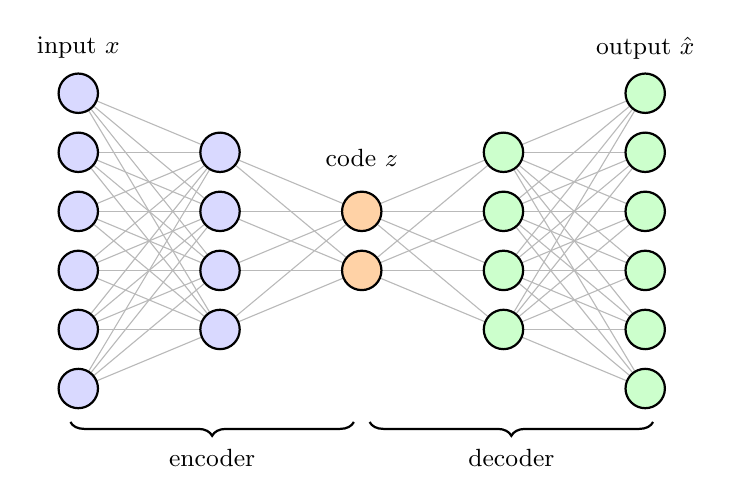
\begin{tikzpicture}[neuron/.style={circle, draw, thick, minimum size=5mm, inner sep=0pt},
    brace/.style={decorate, decoration={brace, amplitude=5pt}, thick}]
  % Layer l sits at x = 1.8l with its n units 0.75 apart, centered on y = 0.
  \foreach \a/\na/\b/\nb in {0/6/1/4, 1/4/2/2, 2/2/3/4, 3/4/4/6}
    \foreach \i in {1,...,\na}
      \foreach \j in {1,...,\nb}
        \draw[gray!55] (1.8*\a, {0.75*(\i-(\na+1)/2)}) -- (1.8*\b, {0.75*(\j-(\nb+1)/2)});
  \foreach \l/\n/\c in {0/6/blue!15, 1/4/blue!15, 2/2/orange!35, 3/4/green!20, 4/6/green!20}
    \foreach \i in {1,...,\n}
      \node[neuron, fill=\c] at (1.8*\l, {0.75*(\i-(\n+1)/2)}) {};
  \node[font=\small] at (0,2.45) {input $x$};
  \node[font=\small] at (3.6,1.05) {code $z$};
  \node[font=\small] at (7.2,2.45) {output $\hat{x}$};
  \draw[brace] (3.5,-2.3) -- node[below=6pt, font=\small] {encoder} (-0.1,-2.3);
  \draw[brace] (7.3,-2.3) -- node[below=6pt, font=\small] {decoder} (3.7,-2.3);
\end{tikzpicture}
